\section{Experimental Result for CIFAR-10}

In the Table \ref{cifar10conf} there is the result for the testing images of CIFAR-10 dataset. Here, each row represents the testing label, each column represents the label produced by the network. For example the cell (1,1) represents that the testing label is airplane and the tagged label is airplane, the cell (1,2) represents that the testing label is airplane and the tagged label is automobile. So, each cell (i,i) where $[i = 1..10]$ represents the correctly tagged labels. Each row consists of 1000 image labels. So the accuracy will be cell$(i,i)/1000$.

%\begin{figure}[h!]
%  \centering
%  \includegraphics[width=0.9\textwidth]{cifar10.PNG}
%  \caption{CIFAR-10 Confusion Matrix}\label{cifar10conf}
%\end{figure}


\begin{table}[!htb] 
 \centering
  \includegraphics[width=0.9\textwidth]{cifar10.PNG}
  \caption{CIFAR-10 Confusion Matrix}
  \label{cifar10conf}
\end{table}


\section{Experimental Result for Multi-Label Image tagging}
To give an overview of the process of inspecting the result of the segmented images, we will need the help of Table \ref{score}. The table is for a single multi-label image. Each $image_{i}$ represents the segmented image from the multi-label image. Each row represents the class scores given by the network. 

\paragraph{Selecting Top-1 Score:}
In this approach we select the top 1 score and its associating label from each segmented image $image_{i}$. Then we increase the frequency of labels for each top 1 score. After that we select the top 4 scoring labels. For example, in the Table \ref{score} the top 1 label for $image_{1}$ would be cat. So we increase the frequency of cat by 1. Similarly for $image_{2}$ again the score for label cat is highest. So frequency of cat will be increased by 1.

%\begin{figure}[h!]
%  \centering
%  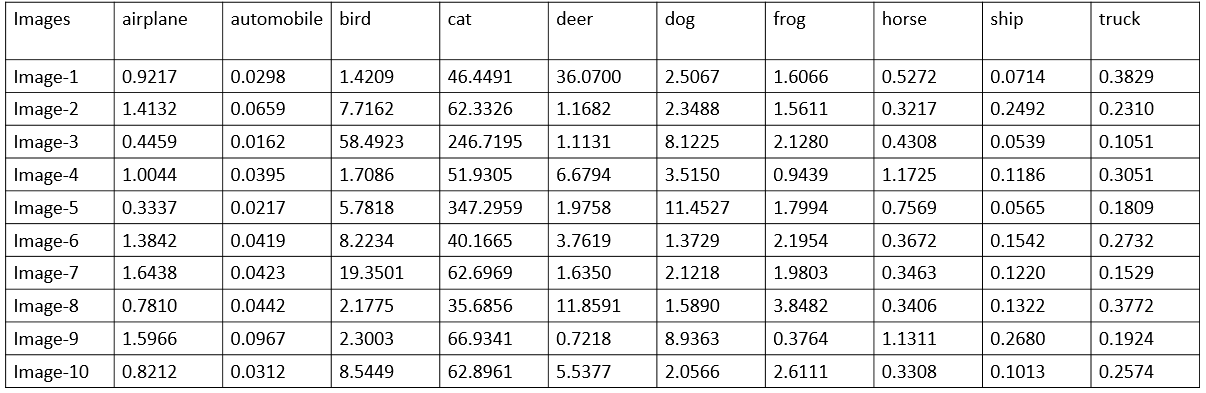
\includegraphics[width=0.9\textwidth]{newresult.PNG}
%  \caption{Scores for the sample image}\label{score}
%\end{figure}

\begin{table}[!htb]
 \centering
  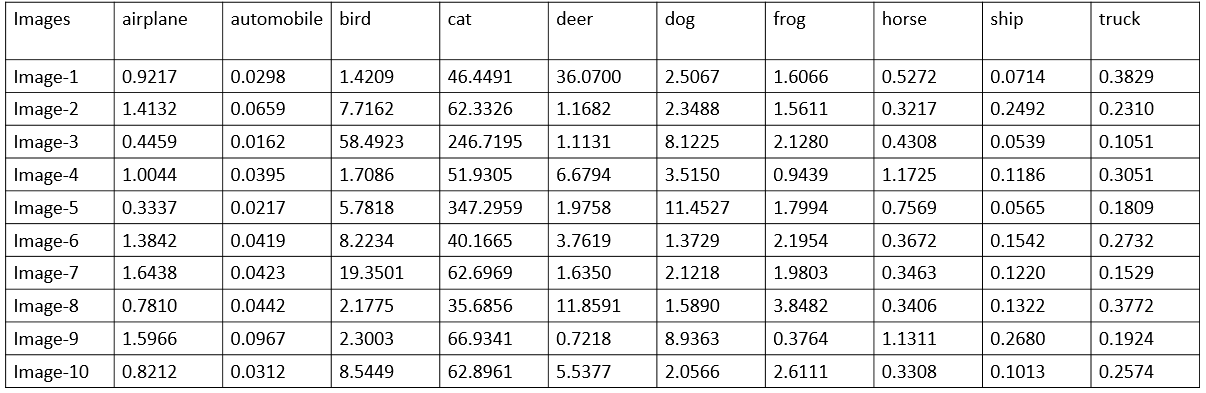
\includegraphics[width=0.9\textwidth]{newresult.PNG}
  \caption{Scores for the sample image}
  \label{score}
\end{table}

\paragraph{Selecting Top-2 Score:}
In this approach we select the top 2 scores and its associating label from each segmented image $image_{i}$. Then we increase the frequency of labels for each top 2 scores. After that we select the top 4 scoring labels.  For example, in the Table \ref{score} the top 2 labels for $image_{1}$ would be cat and deer. So the frequency of cat and deer will be increased by 1.

%\begin{figure}[h!]
%  \centering
%  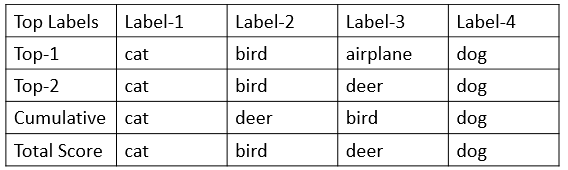
\includegraphics[width=0.9\textwidth]{result_objectness.PNG}
%  \caption{Result for the sample image for Objectness Measures}\label{resobj}
%\end{figure}

\begin{table}[!htb]
\centering
  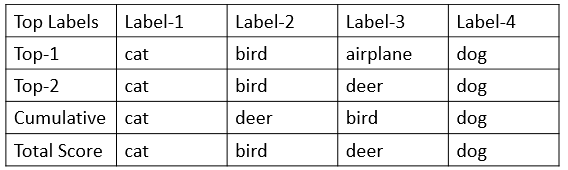
\includegraphics[width=0.9\textwidth]{result_objectness.PNG}
  \caption{Result for the sample image for Objectness Measures}
   \label{resobj}
\end{table}

\paragraph{Selecting Total Score:}
In this approach we just add all scores of each $label_{i}$ for each segmented image $image_{i}$. Then we select the top 4 scoring labels. For example, every class score for every label will be added. So, the score for cat label will be the total score in the column cat. Similarly the score for bird will be the total score in the column bird.

%\begin{figure}[h!]
%  \centering
%  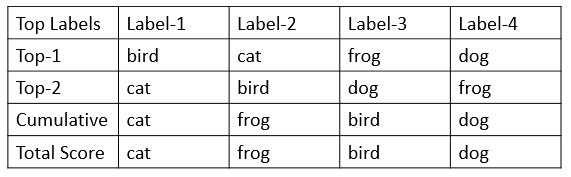
\includegraphics[width=0.9\textwidth]{result_selective.PNG}
%  \caption{Result for the sample image for Selective Search}\label{ressel}
%\end{figure}

\begin{table}[!htb]
\centering
  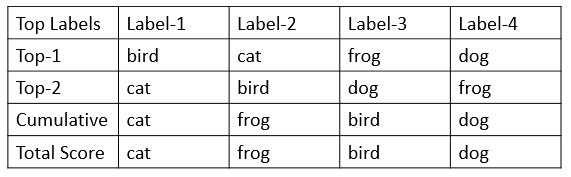
\includegraphics[width=0.9\textwidth]{result_selective.PNG}
  \caption{Result for the sample image for Selective Search}
  \label{ressel}
\end{table}

\paragraph{Selecting Cumulative Percentage:}
Each $label_{i}$ of segmented image $image_{i}$ has the percentage $score_{i} / \sum_{i}{score_{i}}$. We select the top percentage from each segmented image $image_{i}$. We add these percentages for each associated labels and select the top 4 scoring labels. For example for $image_{1}$ the percentage of cat will be $score_{cat} / \sum_{i}{score_{i}}$.\hfill \break

The results for these four approaches for the sample image from Figure \ref{sample_multi_label} is given at Table \ref{resobj} and Table \ref{ressel} \hfill \break


These approaches were repeated in our selected multi label images. The results for Objectness Measure is given in Figure \ref{finobj} and for Selective Search in Figure  \ref{finsel}

\begin{figure}[h!]
  \centering
  \includegraphics[width=0.5\textwidth]{sample_multi_label.PNG}
  \caption{Sample Multi-Label Image}\label{sample_multi_label}
\end{figure}


\begin{figure}[h!]
  \centering
  \includegraphics[width=0.5\textwidth]{Capture3.PNG}
  \caption{Result for multi-label images for Objectness Measures}\label{finobj}
\end{figure}


\begin{figure}[h!]
  \centering
  \includegraphics[width=0.5\textwidth]{Capture4.PNG}
  \caption {Result for multi-label images for Selective Search}\label{finsel}
\end{figure}

\section{Discussion}

The main problem of tagging multi-label images are the training time required. If Convolutional Neural Network is used for tagging multiple labels, then there is a chance that the networks will be very complex. This will require a lot of time to train. Also, if it takes a lot of time to train, then tweaking the network and exploring promising functionalities will require a lot of time. But our Convolutional Neural Network can only tag Single Label images, then we use this network to tag the segmented images provided by Objectness Measures and Selective Search approach. The Convolutional Neural Network we provided is faster to train, so tweaking the network will provide quick result. We got about 57\% accuracy using the Selective Search approach shown in \ref{finsel}. So, we can expect that if we increase the capability of our network, this accuracy will be much higher.

